%%%%%%%%%%%%%%%%%%%%%%%%%%% Figure 6 General curvilinear model %%%%%%%%%%%%%%%%%%%%
\begin{figure}[t]
 \begin{center}
  \begin{pspicture}(0,0)(15,11)
% Include graphs
   \rput[b](7.5,0.0){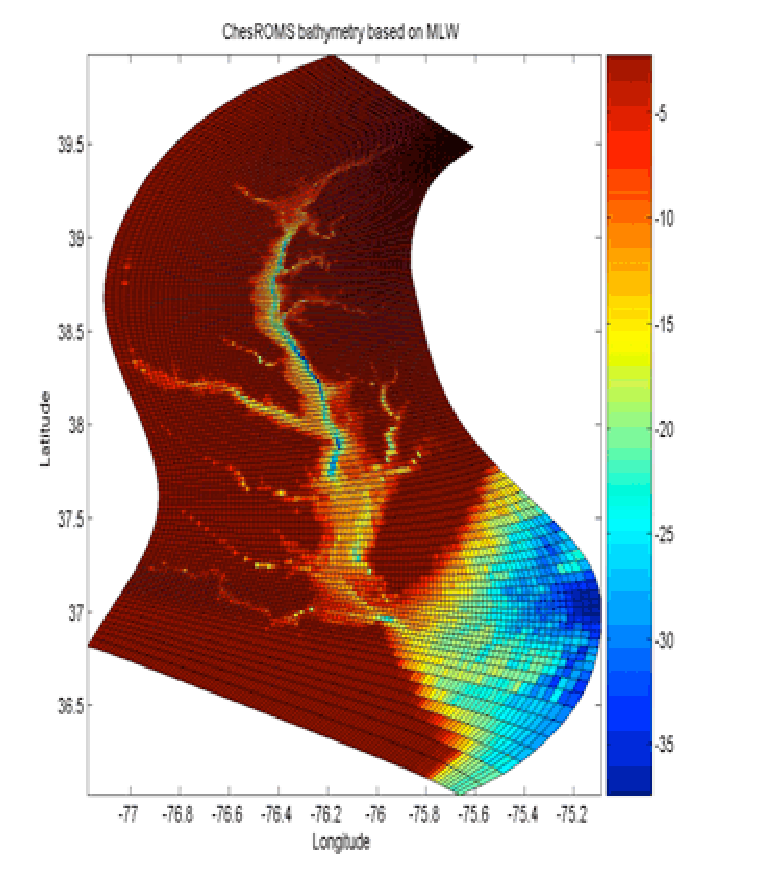
\includegraphics[height=11cm]{ChesROMS_grid}}
  \end{pspicture}
  \caption{\small Examples of a curvilinear grid showing the curvilinear grid used for the Cheasapeake Bay model ChesROMS. Note how the grids follows the land/sea matrix, thus minimizing the number of ``dry'' points. Likewise, note how the grid size varies in space.} 
  \label{fig:curvil}
 \end{center}
\end{figure}

